\subsection{Interpolazione Lagrangiana composita}

Una miglioria che è possibile fare all'interpolazione Lagrangiana, è quella di introdurre un \textbf{interpolatore continuo dato dall'unione di tanti interpolatori Lagrangiani di basso ordine}, ovvero $k \ll n$.

\highspace
Tali singoli interpolatori locali sono costruiti sugli intervalli disgiunti $I_{j}$ ognuno composto da $k+1$ nodi e di lunghezza $H = kh$:

\begin{figure}[!htp]
	\centering
	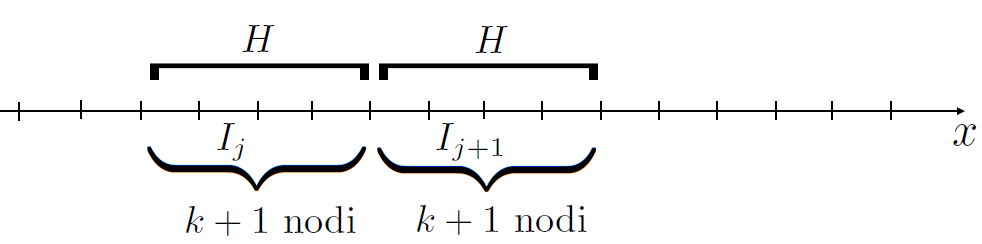
\includegraphics[width=0.7\linewidth]{img/interpolazione-lagrangiana-composita-1.png}
\end{figure}

\noindent
Tale interpolatore globale, chiamato \definition{interpolazione Lagrangiana composita}, viene indicato con $\prod_{k}^{H}\left(x\right)$. Se si vuole enfatizzare che l'interpolatore è stato costruito per approssimare una certa funzione $f$, allora si utilizza la notazione $\prod_{k}^{H} f\left(x\right)$.

\begin{examplebox}[: interpolatore Lagrangiano composito lineare]
	Si consideri il caso $k=1$. La funzione rappresentata in linea continua è:
	\begin{equation*}
		f\left(x\right) = x^{2} + \dfrac{10}{\left(\sin\left(x\right)+1.2\right)}
	\end{equation*}
	Ed il suo interpolatore lineare composito rappresentato con la linea tratteggiata:
	\begin{equation*}
		\displaystyle\prod_{1}^{H}f\left(x\right)
	\end{equation*}
	\begin{center}
		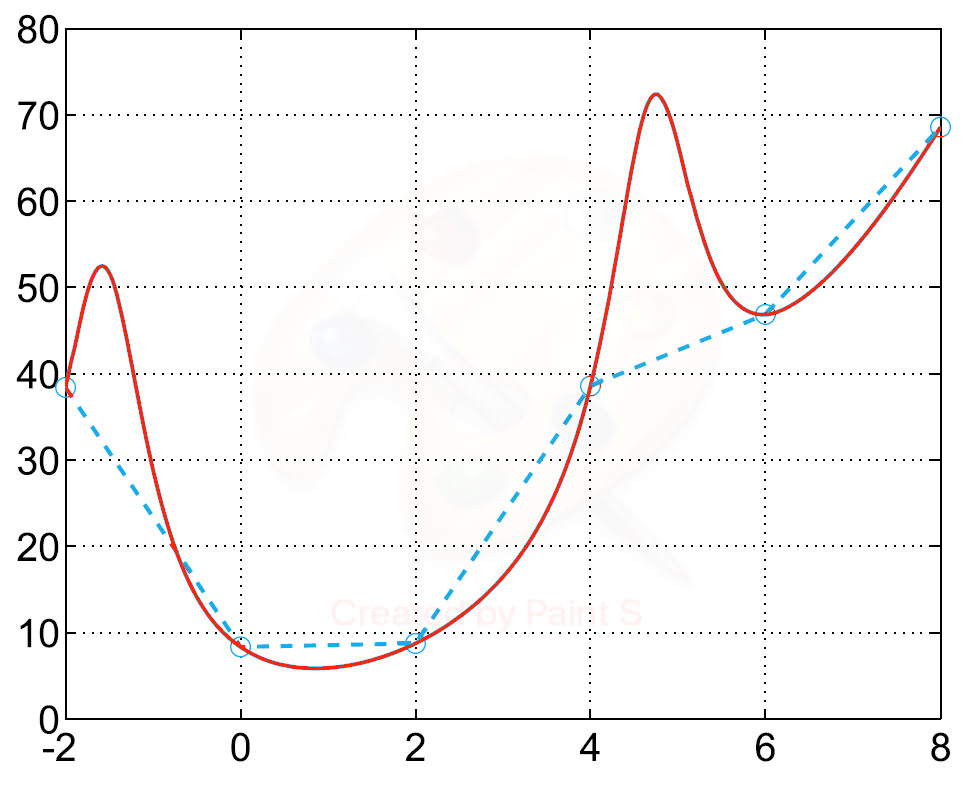
\includegraphics[width=.6\textwidth]{img/interpolazione-lagrangiana-composita-2.png}
	\end{center}
	
	\noindent
	Vista la sua semplicità, questo interpolatore è molto utilizzato nelle applicazioni.
\end{examplebox}

\newpage

\subsubsection{Accuratezza (errore) e convergenza dell'interpolatore Lagrangiano composito}

A differenza dell'interpolazione Lagrangiana, all'aumentare del numero di informazioni $n+1$ che si hanno a disposizione, l'accuratezza dell'interpolatore Lagrangiano composito subisce un \emph{miglioramento}.

\highspace
All'aumentare del valore di $n$, verranno aumentati anche il numero di intervalli $I_{j}$ su cui costruire gli interpolatori Lagrangiani locali, \textbf{senza variare il gradi locale $k$ che rimarrà costante}. Questa tecnica riesce ad evitare il fenomeno di Runge, ovverosia che l'interpolatore Lagrangiano non raggiunge la convergenza.

\highspace
Riguardo alla convergenza, si introduce l'\textbf{errore puntuale}:
\begin{equation}
	E_{k}^{H}f\left(x\right) = f\left(x\right) - \displaystyle\prod_{k}^{H}f\left(x\right)
\end{equation}
Il quale è dato dal massimo degli errori degli interpolatori Lagrangiani di grado $k$ su ogni $I_{j}$. In caso di nodi equispaziati, si ottiene che la \definition{stima dell'errore dell'interpolatore Lagrangiano composito} tende a zero nel caso in cui $H$ tende a zero:
\begin{equation}\label{eq: stima dell'errore interpolatore Lagrangiano composito}
	\begin{array}{rcl}
		\underset{x \in I}{\max} \left| E_{k}^{H} f\left(x\right) \right| & \le & \underset{j}{\max} \dfrac{\underset{x \in I_{j}}{\max} \left|f^{\left(k+1\right)}\left(x\right)\right|}{4\left(k+1\right)} \cdot h^{\left(k+1\right)} \\ [1.5em]
		%
		&\le& \dfrac{\underset{x \in I}{\max} \left|f^{\left(k+1\right)}\left(x\right)\right|}{4\left(k+1\right)} \cdot h^{\left(k+1\right)} \\ [1.5em]
		%
		&& \text{sostituendo } h \text{ con } \dfrac{H}{k} \\ [1.5em]
		%
		&\le& \underbrace{\dfrac{\underset{x \in I}{\max} \left|f^{\left(k+1\right)}\left(x\right)\right|}{4\left(k+1\right)k^{\left(k+1\right)}}}_{\text{Indipendente da }H} \cdot H^{\left(k+1\right)}
	\end{array}
\end{equation}
Oltre ad un errore, questo dimostra la \definition{convergenza dell'interpolatore Lagrangiano composito}.

\newpage

\begin{flushleft}
	\textcolor{Green3}{\faIcon{question-circle} \textbf{Se $H$ e $k$ sono importanti, come devono essere scelti?}}
\end{flushleft}
Dipende dall'origine dei dati:
\begin{itemize}
	\item Se i dati provengono da una funzione $f\left(x\right)$ nota sull'intervallo $\left[a,b\right]$ che genera $y_{i} = f\left(x_{i}\right)$ con $i = 0, \dots, n$, allora:
	\begin{itemize}
		\item Si \textbf{decide il valore di} $k$ da utilizzare cercando di non superare il valore $3$ per non incorrere nel fenomeno di Runge (non convergenza!);
		
		\item Si \textbf{sceglie il valore dell'ampiezza degli intervalli} $H$ in modo da avere l'errore desiderato in base alla stima dell'errore riportato nell'equazione \ref{eq: stima dell'errore interpolatore Lagrangiano composito};
		
		\item Si \textbf{partiziona l'intervallo} $\left[a,b\right]$ in intervallo di ampiezza $H$ e su \textbf{ognuno di essi si considerano $k+1$ nodi}.
	\end{itemize}
	
	\item Se i dati provengono da misure, il numero di questi $n+1$ è fissato. Per cui le operazioni da fare possono essere una delle seguenti:
	\begin{itemize}
		\item Un'\definition{interpolazione composita lineare}:
		\begin{equation*}
			k=1 \hspace{2em} H = \dfrac{\left(b-a\right)}{n}
		\end{equation*}
		
		\item Un'\definition{interpolazione composita quadratica}:
		\begin{equation*}
			k = 2 \hspace{2em} H = \dfrac{2\left(b-a\right)}{n}
		\end{equation*}
	\end{itemize}
\end{itemize}